\section{Views} 
\label{sec:views}

\subsection{Logic View}
A simple version of the logic view was made, because it is hard to foresee all
help classes and states prior to the development process. 
\begin{center}
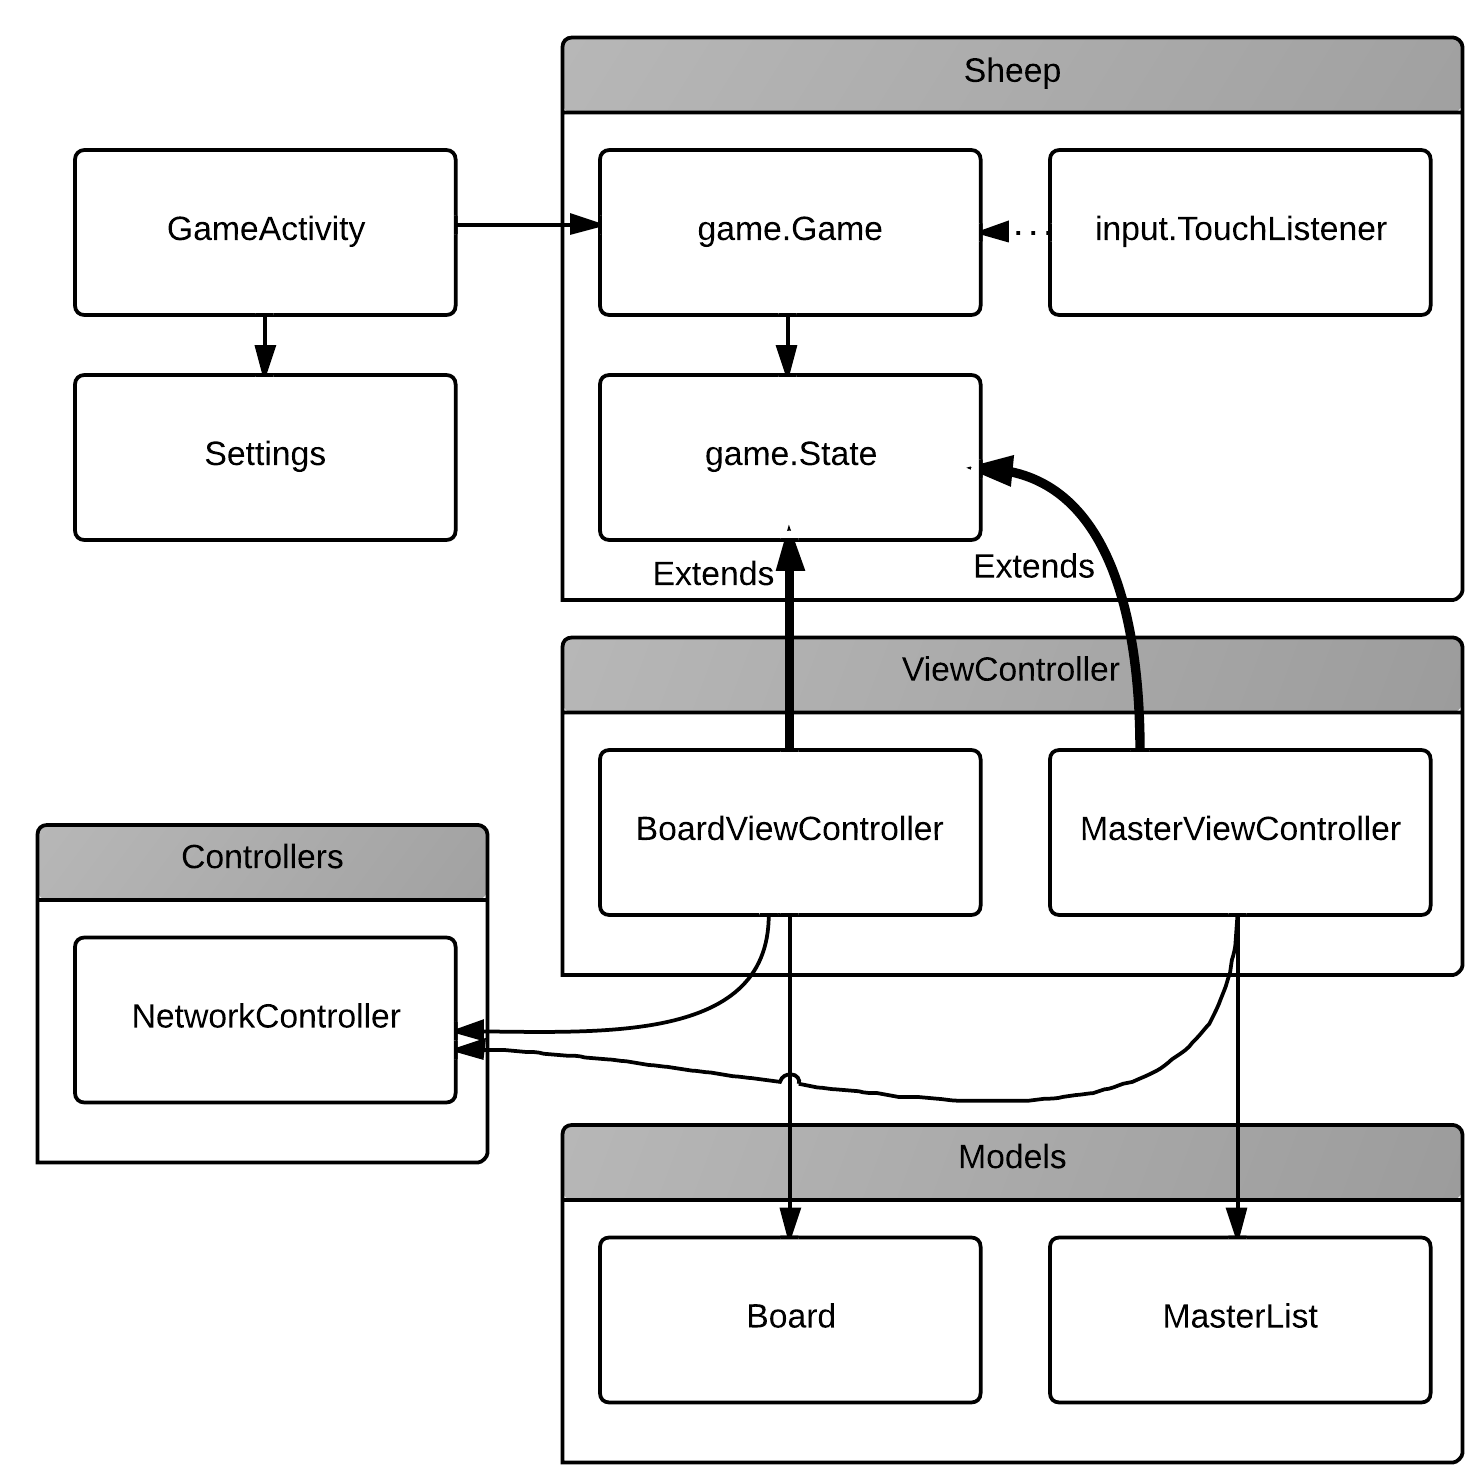
\includegraphics[clip=true, width=0.9 \textwidth]{assets/LogicView.png}
\captionof{figure}{Logic View}
\label{ref:gantt}
\end{center}

\subsection{Development View}
The development view is a hierarchy of layers containing assets such as the
graphics, the game logic including handeling of states and input, the Sheep
framework that is a typical help-framework, and the Android SDK taking care
of the network and the base system.
\begin{center}
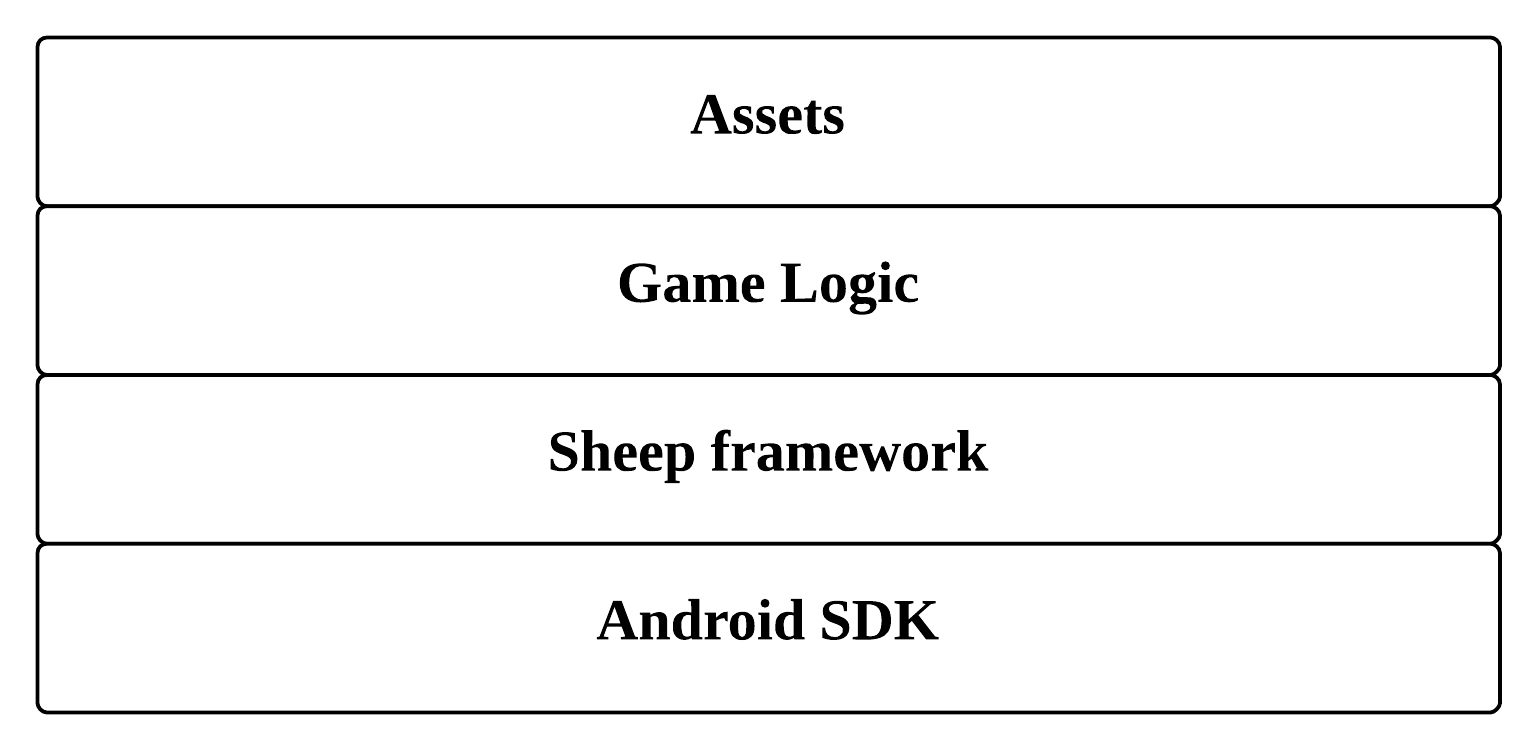
\includegraphics[clip=true, width=0.9 \textwidth]{assets/DevelopmentView.png}
\captionof{figure}{Development View}
\label{ref:gantt}
\end{center}

\subsection{Process View}
The process view shows the procedure in the game. How connections are made
between states and screens. \\\\
The menu screen is the start point of this application, where there are options
to navigate to either the authentication- or the settings screens.
From the authentication screen, the user can log in or out to the admin screen.
\\\\
The main menu screen also provides the option to join a new game, and the user
is then transferred to the game screen which has listeners for notification
states. The game ended screen returns to the main menu.
\begin{center}
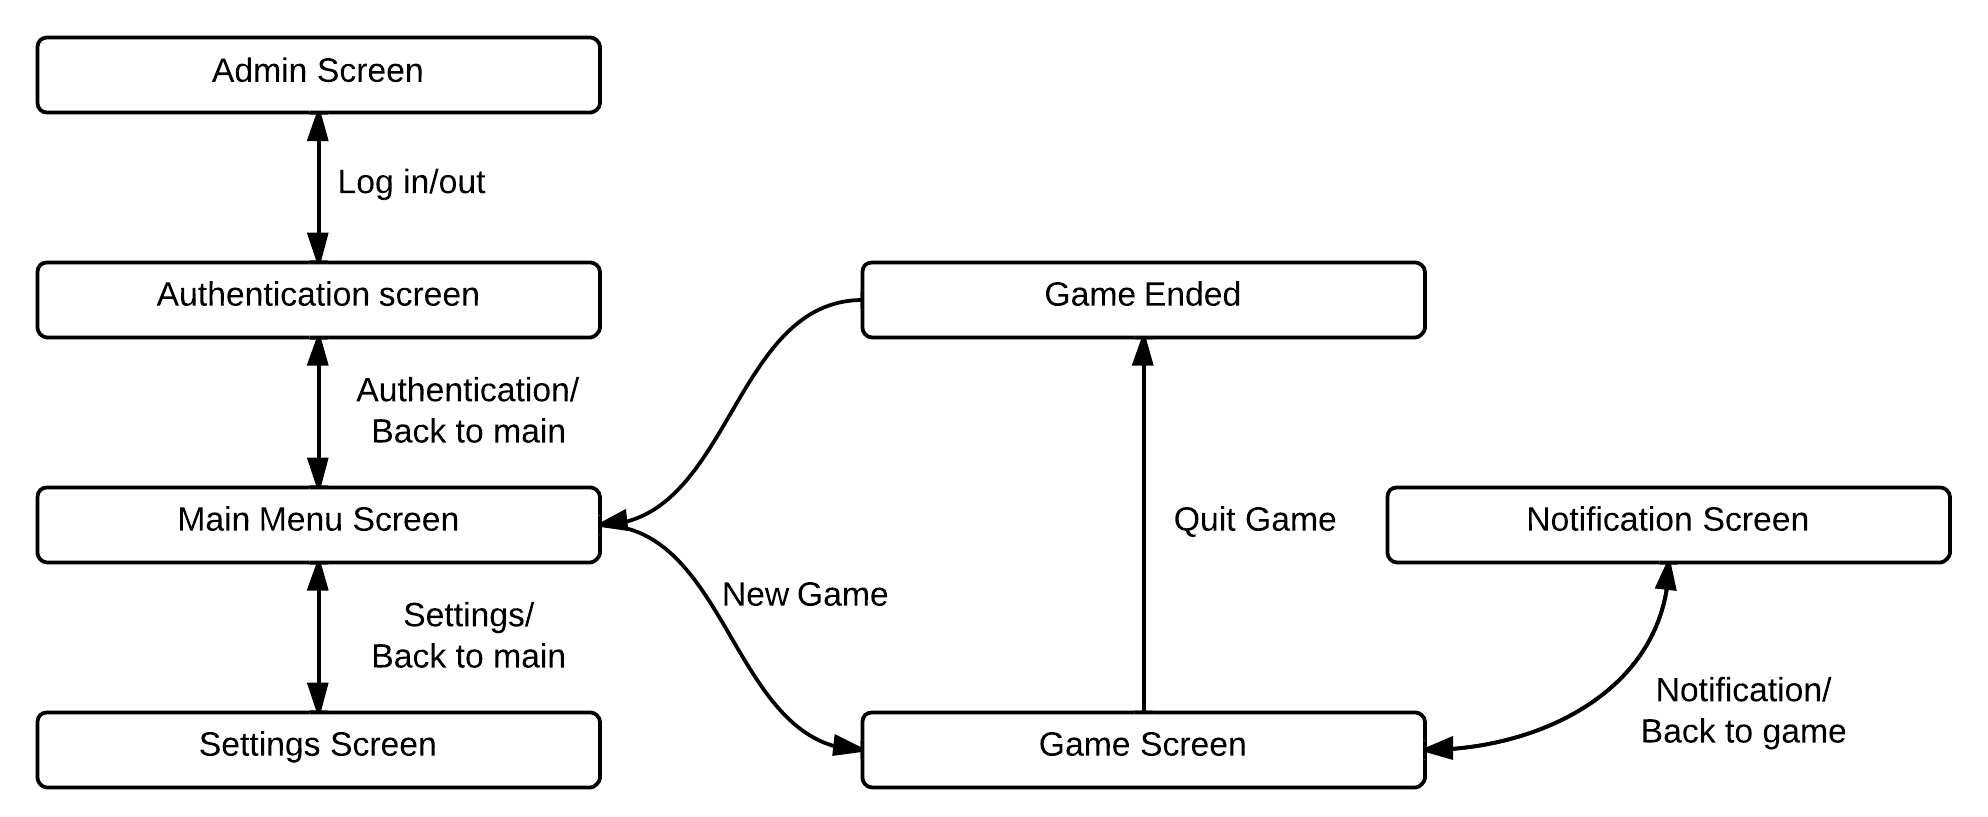
\includegraphics[clip=true, width=0.9 \textwidth]{assets/ProcessView.png}
\captionof{figure}{Process View}
\label{ref:gantt}
\end{center}

\subsection{Physical View}
The client are divided into the shuffled board, the game logic, game quiery and
the session info. The server includes the current words that contains the
master list returns to the shuffled board. The game state is a two-way
communication with logic, and the same hold for the usable words. The connection
pool relates to the session info to ensure the connection between client and server.
\begin{center}
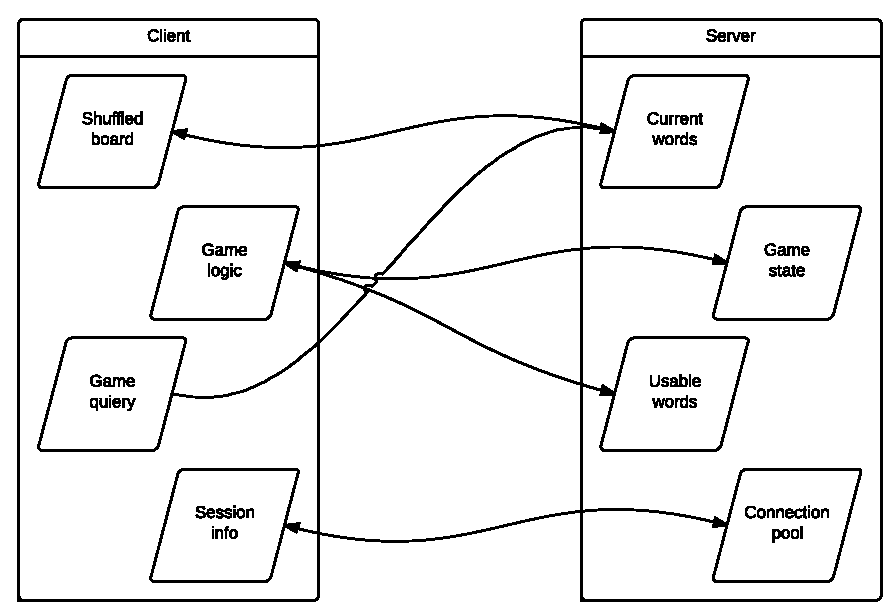
\includegraphics[clip=true, width=0.9 \textwidth]{assets/PhysicalView.pdf}
\captionof{figure}{Physical View}
\label{ref:gantt}
\end{center}
